\chapter{Literature Review}

\section{Problem Area Contextualisation}
Due to advancements in the processing power of embedded systems and developments in small-scale, low-cost \acrshort{uav}s, the topic of multi-\acrshort{uav} enabled networks has become a focus of research with aims to practical implementations in recent years. Other relevant developments in networking include the development of communication schemes such as \acrlong{ofdm} (\acrshort{ofdm}), which is a spectrally efficient modulation scheme for \acrshort{4g} as well as \acrshort{noma} for \acrshort{5g} wireless communication standards. 

In regions where there is no network infrastructure, aerial alternatives that make use of \acrshort{uav}s, \acrlong{hap}s (\acrshort{hap}s) or both \acrshort{uav}s and \acrshort{hap}s can be utilised to serve the purpose of traditional network infrastructure. 
Such environments may include regions where there is no conventional network infrastructure due to the infrastructure being damaged or destroyed as a result of a natural disaster or where the region is too remote with terrain that is too inhospitable to feasibly construct the network infrastructure required for modern connectivity and security demands. This application is illustrated in Fig. \ref{fig:uav_public_safety}, which has been reproduced from \cite{saad_wireless_2020}. 

\begin{figure} [ht!]
    \centering
    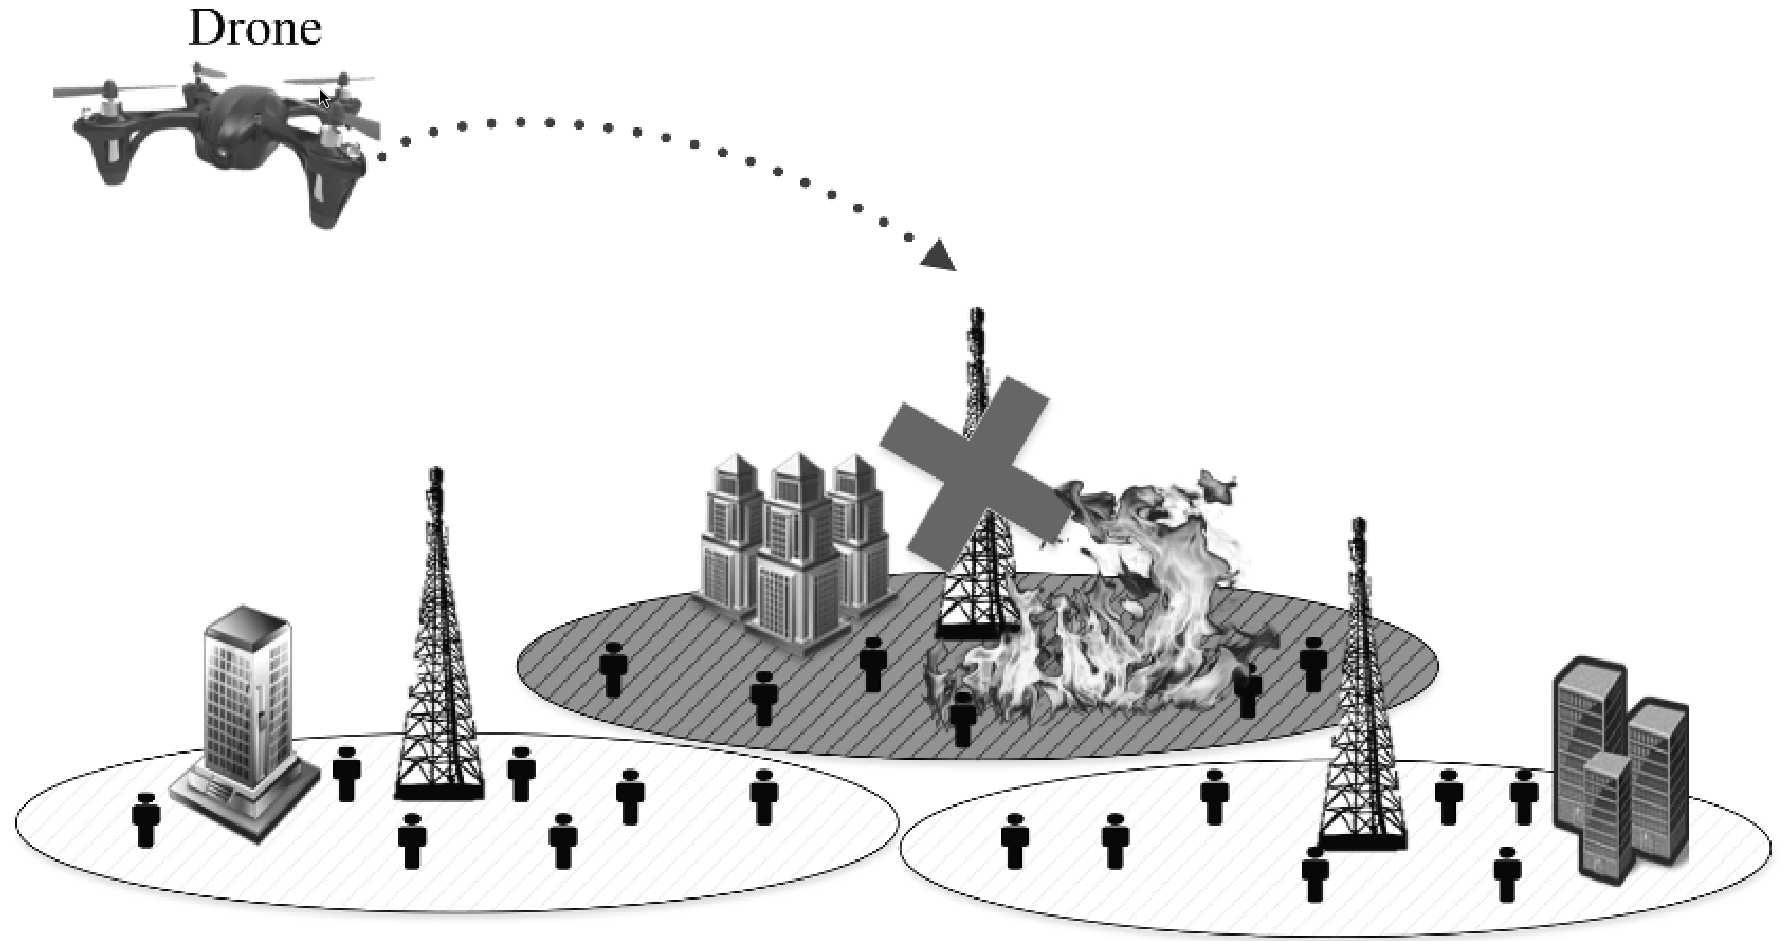
\includegraphics[width=0.75\textwidth]{figures/uav_public_safety_scenario.png}
    \caption{\acrshort{uav}s Acting as Network Infrastructure in a Disaster Scenario}
    \label{fig:uav_public_safety}
\end{figure}

Different approaches to this problem involving optimisation techniques will optimise a particular parameter as part of the system and treat others as constraints such that the best system performance with respect to the objective is achieved. 
This involves the design of algorithms based on closed-form mathematical derivations as well as numerical methods such as machine learning. 
Different system architectures are explored in the literature on this topic, which include \acrshort{uav}-\acrshort{hap}s aerial networks \cite{zhang_one_2025, ji_joint_2023, azizi_exploring_2024}, multi-\acrshort{uav} networks \cite{mu_security_2021, jeong_quantum_2025} and \acrshort{hap}-enabled networks. 

Optical communications exist and can be used effectively for secure wireless communications, however, the focus of this thesis and literature review is on radio communications as radio communications are more commonly used for wireless communications. 

Both quantum \cite{jeong_quantum_2025, silvirianti_layerwise_2024, li_intelligent_2021, saravanan_optimizing_2024} and classical optimisation techniques with applications to \acrshort{uav}-enabled networks have been explored in the literature. 

\section{Aerial Communications}
Airborne networks provide some benefits over terrestrial ones. One major benefit of airborne networks involving the use of \acrshort{uav}s for communications is that the networking platforms can reach higher altitudes than standard radio towers and their position can be adjusted dynamically to optimise their \acrfull{los} for air-to-air, air-to-ground and ground-to-air communications links. 
This is a substantial benefit over ground-based networks in regions where a clear \acrshort{los} cannot be attained easily, such as a dense urban environment, woodlands, etc., where communications links are otherwise very difficult to establish without the use of airborne communications platforms such as \acrshort{uav}s \cite{namuduri_uav_2017}.

\acrshort{uav}s can serve a variety of purposes as communications platforms. \acrshort{uav}s acting as a \acrfull{lap} oftentimes will have shorter missions and are more suitable for short-term, dynamic coverage, whereas \acrshort{hap}s are better utilised for longer-term missions \cite{namuduri_uav_2017}.

\acrshort{uav}s can serve a variety of purposes in an airborne communications network, such as acting as \acrshort{bs}s, relays, wireless \acrfull{ue} and others \cite{namuduri_uav_2017, saad_wireless_2020}.

\acrshort{uav}s can be used for jamming signals with a noise signature that is known by the friendly nodes in the network, such as \acrshort{gu}s, \acrshort{hap}s, \acrshort{bs}s, etc. and is unknown to eavesdroppers. These interfering signals can be used to mask the communication signals through a channel in a way that can be decoded by friendly actors in the network and serve as a challenge for eavesdroppers to be able to interpret the data being transmitted through an airborne network \cite{zhang_one_2025, lohan_secrecy-aware_2022}. 

%\subsection{\acrshort{uav}-\acrshort{hap}s Communications}
\subsection{\texorpdfstring{\acrshort{uav}-\acrshort{hap}s}{UAV-HAPs} Communications}
Both LAP and \acrshort{hap} \acrshort{uav}s can be used together \cite{zhang_energy-efficient_2024, ji_joint_2023, zhang_one_2025, qin_secure_2023} to create a network in which longer-term, more stable network coverage and communications are provided by the \acrshort{hap} portion of the system and the shorter-term, lower altitude communications are handled by the LAP portion of the system. 

Some challenges involving this kind of airborne network architecture involve the multiple degrees of freedom introduced by both \acrshort{hap} and LAP \acrshort{uav}s. This requires the use of optimisation algorithms being developed for various parameters involving both systems such that the entire system is performing as desired, i.e., with the most optimal outcomes depending on the focus of the network. 
Some examples of aspects of the system that require optimisation are the \acrshort{hap}/LAP deployment, energy efficiency of both \acrshort{hap}s and LAPs, resource allocation and secrecy \cite{zhang_one_2025}.
\begin{figure}[ht]
    \centering
    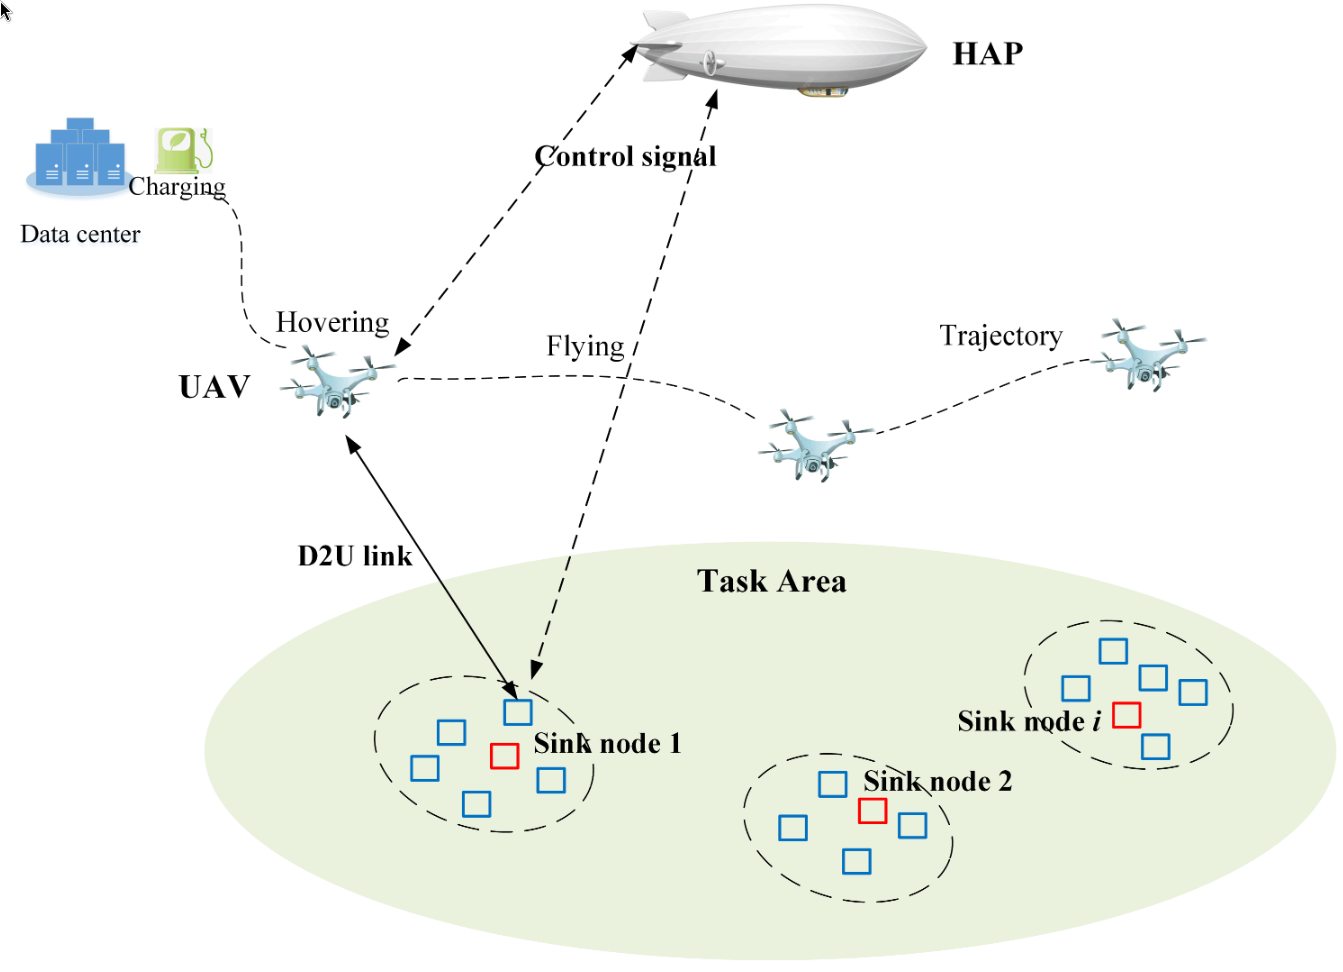
\includegraphics[width=0.75\textwidth]{figures/uav_hap_network_energy_efficient.png}
    \caption{Illustration of a \acrshort{uav}-\acrshort{hap} Network Model}
    \label{fig:energy_efficient_uav_hap_zhao}
\end{figure}
An illustration of a \acrshort{uav}-\acrshort{hap} network reproduced from \cite{zhao_energy_2023} is shown in Fig. \ref{fig:energy_efficient_uav_hap_zhao}, where \acrshort{uav}s and \acrshort{hap}s are integrated as an airborne network over a given task area to form device-to-\acrshort{uav} communications. These device-to-\acrshort{uav} communication links provide a means of communication between terrestrial terminal devices (\acrshort{td}s) or ground users (\acrshort{gu}s) in sink nodes. 

\subsection{\texorpdfstring{\acrshort{uav}s as Aerial \acrshort{bs}s}{UAVs as Aerial BSs}}
In the case of a \acrshort{uav} serving as an aerial \acrshort{bs}, the \acrshort{uav} itself is the provider of wireless communication services. For purposes such as this, the \acrshort{uav}s behave as low-altitude platforms (\acrshort{lap}s) and thus have a shorter mission time than \acrshort{hap}s or terrestrial \acrshort{bs}s. 

%Fig. \ref{fig:uav_aerial_bs_silvirianti} is taken from \cite{silvirianti_layerwise_2024} and depicts a wireless communications system in which \acrshort{uav}s act as aerial BSs in a network. 
%\begin{figure}[ht]
%    \centering
%    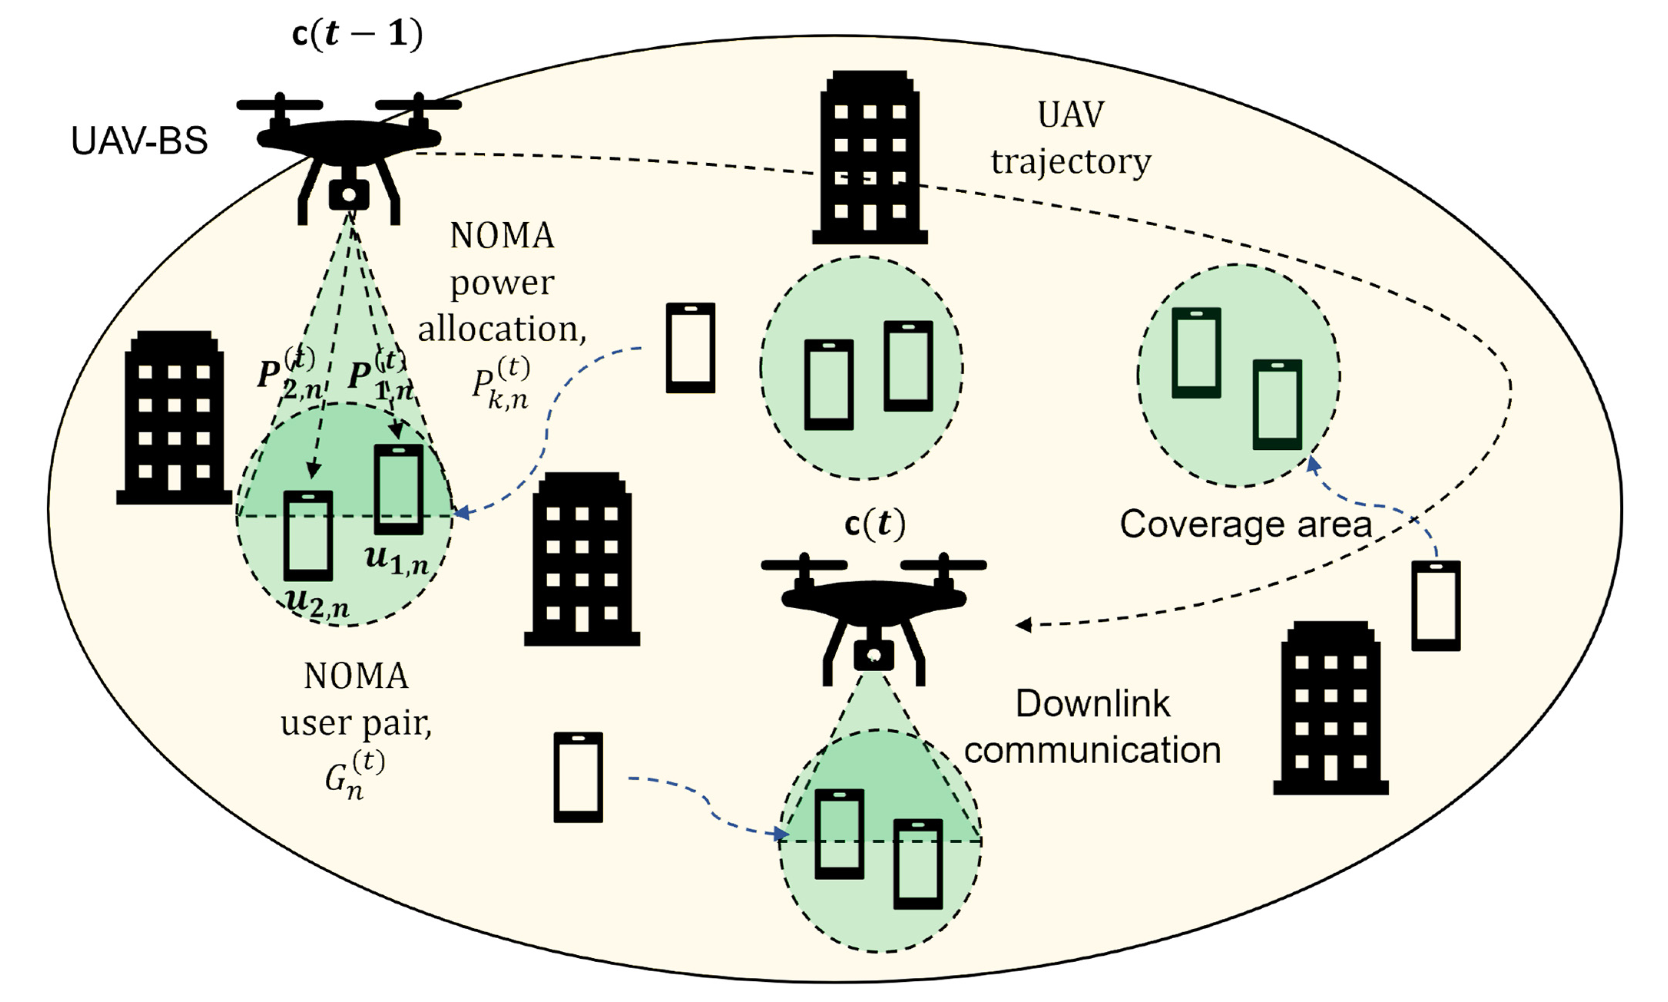
\includegraphics[width=0.75\textwidth]{figures/uav_as_aerial_bs_silviratani_et_al.png}
%    \caption{Network in which \acrshort{uav}s act as Aerial BSs to Provide Coverage to \acrshort{gu}s}
%    \label{fig:uav_aerial_bs_silvirianti}
%\end{figure}
For network architectures like this, the deployment will constantly be changing and thus, typically requires some optimisation of the \acrshort{uav} deployment. 
This constantly changing positioning and deployment model also introduces a need for a channel model that can accurately describe this form of \acrshort{bs} \cite{saad_wireless_2020}. 

\subsection{\texorpdfstring{\acrshort{uav}s}{UAVs} as Relays}
\acrshort{uav}s can be used to extend the range of coverage for a terrestrial or airborne network by serving as network relays between \acrshort{bs}s \cite{zhang_energy-efficient_2024, namuduri_uav_2017, saad_wireless_2020}. 

Fig. \ref{fig:uav_as_relay_namuduri} is a diagram reproduced from \cite{namuduri_mobile_nodate} depicting a \acrshort{uav} serving as a relay between two terrestrial \acrshort{bs}s. 
\begin{figure}[ht]
    \centering
    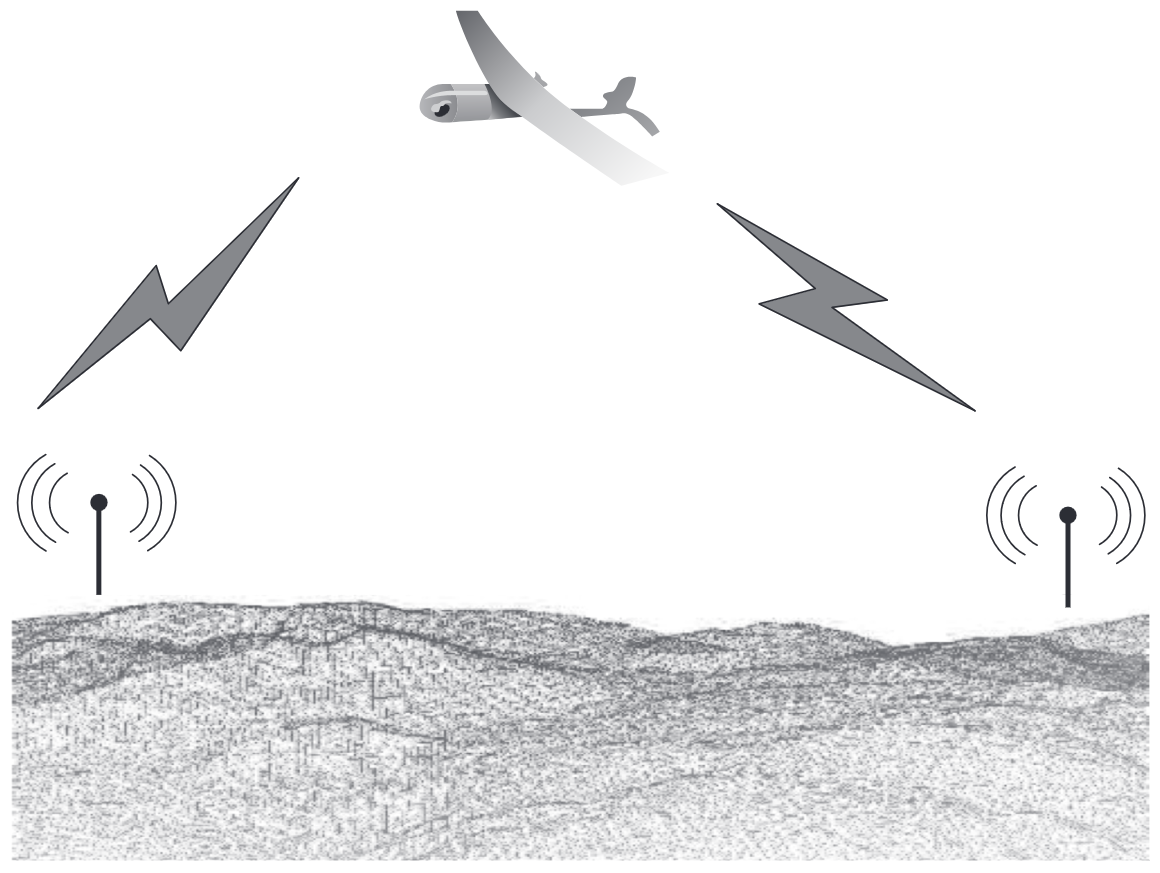
\includegraphics[width=0.75\textwidth]{figures/uav_as_relay_saad_textbook.png}
    \caption{\acrshort{uav} Acting as a Relay Between 2 \acrshort{bs}s}
    \label{fig:uav_as_relay_namuduri}
\end{figure}
\acrshort{uav}s acting as relays for a network can be used to overcome challenges involving poor LoS between other links in a network due to their ability to overcome environmental obstacles dynamically in ways that terrestrial \acrshort{bs}s cannot. 

The use of \acrshort{uav}s as relays does present its own set of challenges, however. Some of these include the necessity to adapt existing relaying mechanisms or to devise novel relaying schemes. 
To ensure proper relaying is achieved, the information related to the control systems of the \acrshort{uav}s, such as their position, altitude, environmental conditions, available resources, etc. must be communicated and known by other \acrshort{uav}s that are directly communicating with it within the network \cite{saad_wireless_2020}. 
Air-to-air links in particular have changing propagation environments, which will be changing frequently as the \acrshort{uav} relays are adjusting their positions and altitude as part of any given mission. 
Multi-hop \acrshort{uav} relays for air-to-air links require the use of dynamic routing algorithms based on the control and communications data from the \acrshort{uav}s in the network, which can be quite challenging to implement on small-scale embedded systems frequently used in small-scale \acrshort{uav}s \cite{saad_wireless_2020}. 

%\subsection{\acrshort{uav}s as \acrshort{ue}s}
\subsection{\texorpdfstring{\acrshort{uav}s as \acrshort{ue}s}{UAVs as UEs}}
\acrshort{uav}s may act as user equipment (\acrshort{ue}) to communicate with existing wireless communication networks, such as WiFi or cellular networks. 
A key challenge involving \acrshort{uav}s as wireless \acrshort{ue}s is that existing terrestrial \acrshort{bs}s have been optimised and designed to provide the best coverage to \acrshort{gu}s rather than airborne \acrshort{ue}s. This has been achieved by designing the main antennae lobes on such \acrshort{bs}s such that they're pointing downwards towards \acrshort{gu}s \cite{saad_wireless_2020}. 
Furthermore, \acrshort{gu}s and \acrshort{uav} \acrshort{ue}s must be differentiated by the network operators to distinguish both classes of user, which has not been a commonly implemented mechanism in conventional networking technologies for \acrshort{ue}s. 

Some applications of cellular-connected \acrshort{uav}-\acrshort{ue}s are presented in Fig. \ref{fig:uav_ue_applications}, which has been adapted from \cite{challita_machine_2019}. 

\begin{figure}[ht!]
   \centering
       \subfigure[\acrshort{uav}-\acrshort{ue}s used in Intelligent Transport Systems]{\label{uav_ue_transport_challita}
           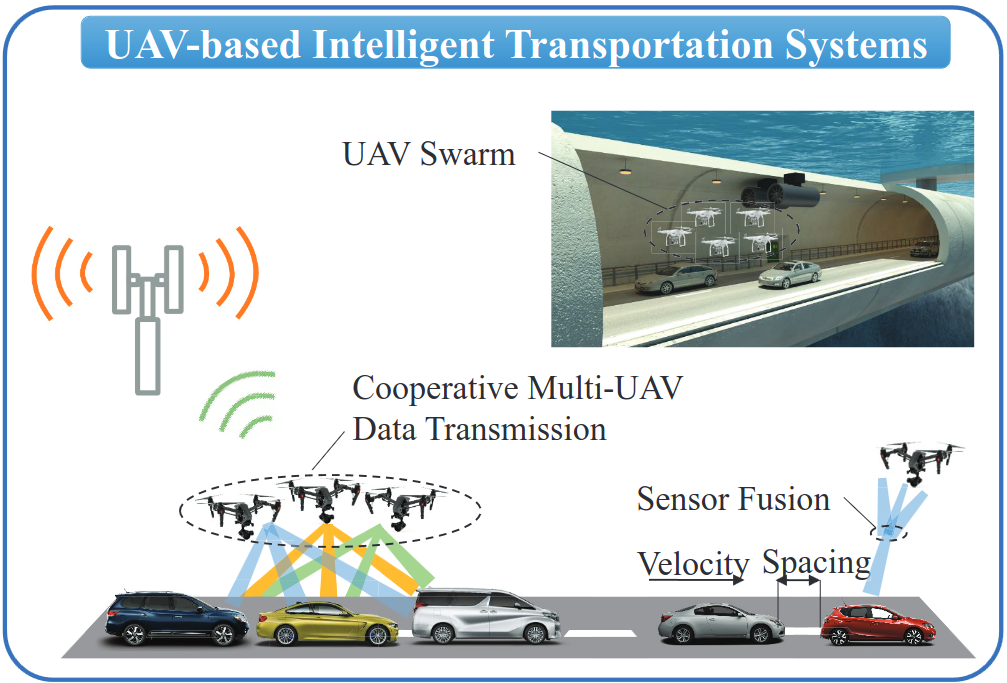
\includegraphics[height=0.2\textheight]{figures/uav_ue_transportation.png}
       }
       \hspace{1mm}
    \subfigure[\acrshort{uav}-\acrshort{ue}s used in Delivery Systems]{\label{uav_ue_delivery_challita}
           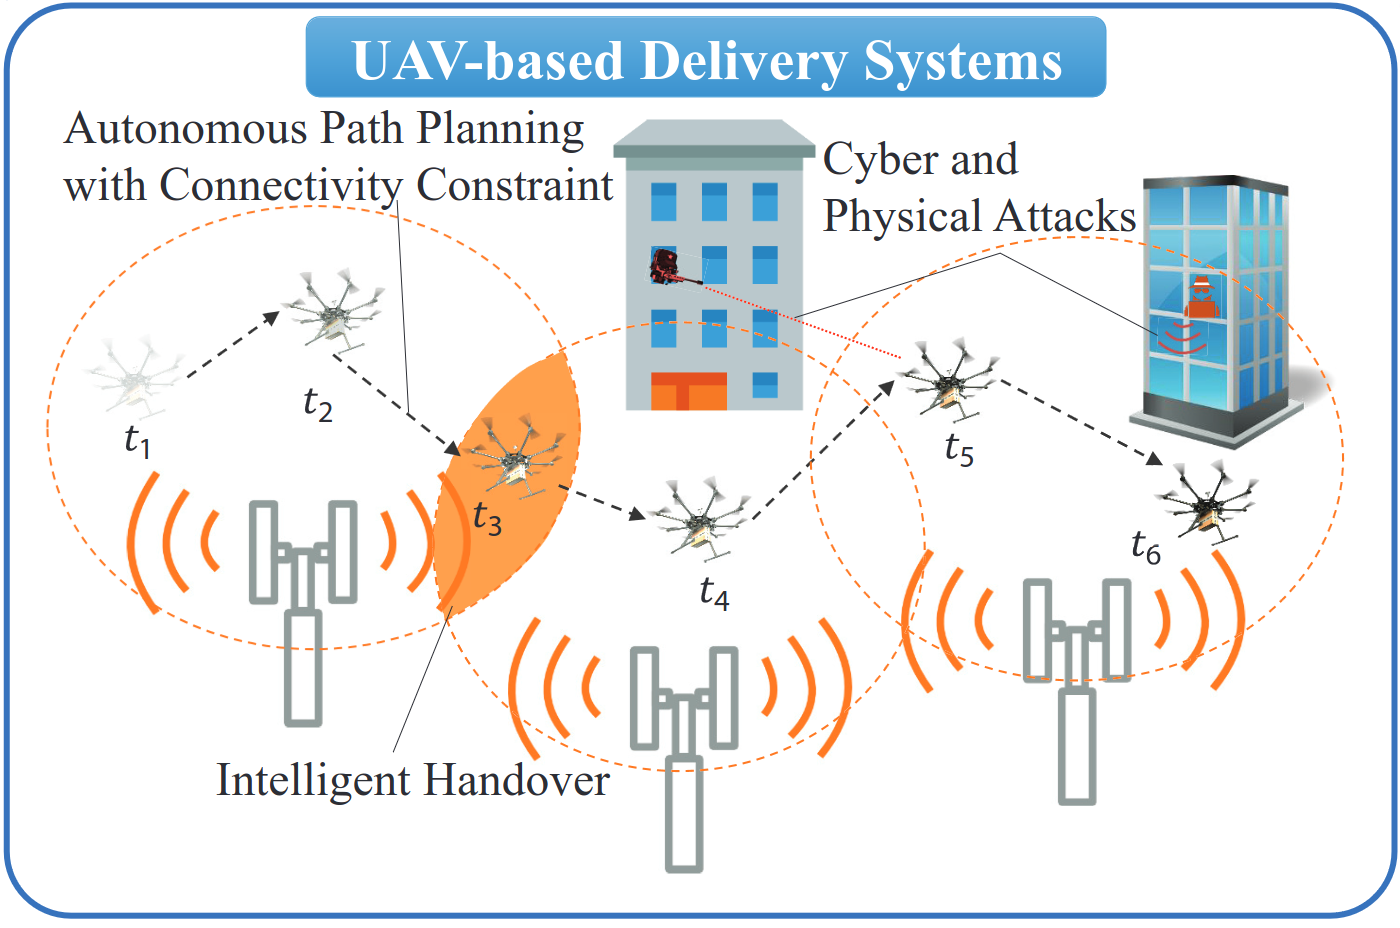
\includegraphics[height=0.2\textheight]{figures/uav_ue_delivery.png}
       }
       \hspace{1mm}
    \subfigure[\acrshort{uav}-\acrshort{ue}s used for Multimedia Streaming]{\label{uav_ue_multimedia_challita}
            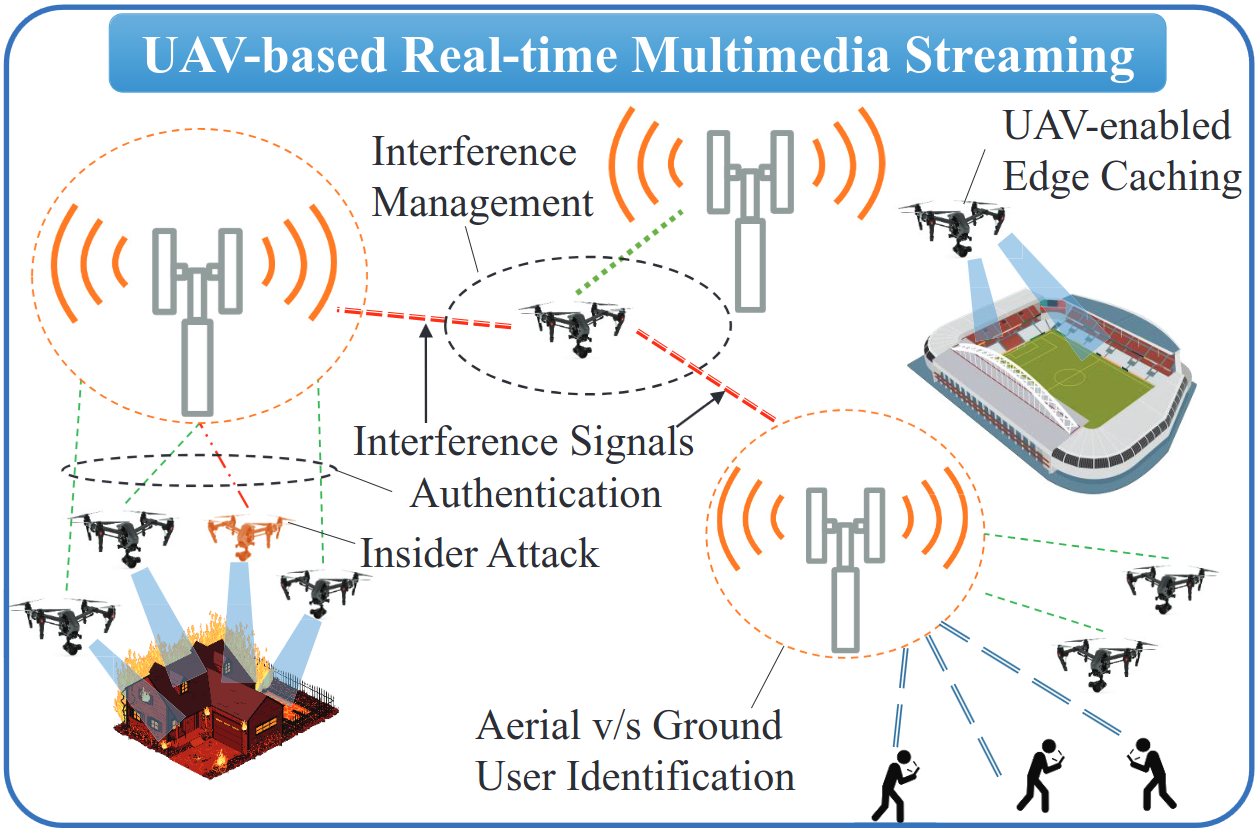
\includegraphics[height=0.2\textheight]{figures/uav_ue_multimedia.png}
        }
       \caption{\acrshort{uav}-\acrshort{ue}s used in Various Systems}
       \label{fig:uav_ue_applications}
\end{figure} 
Cellular-connected \acrshort{uav}s provide beyond \acrshort{los} control, low latency, real-time communication, wide levels of coverage and robust security \cite{challita_machine_2019}, which is advantaged over \acrshort{uav} \acrshort{ue}s connected to a network over short-range communication schemes such as WiFi or Bluetooth. 

\subsection{\texorpdfstring{Ad-Hoc \acrshort{uav}}{Ad-Hoc UAV} Networks}
Mobile ad hoc networks (\acrshort{manet}s) are self-organising networks that are formed by mobile nodes \cite{namuduri_mobile_nodate, namuduri_uav_2017, sahingoz_mobile_2013}. This literature review focuses particularly on \acrshort{uav}-enabled \acrshort{manet}s, however, other forms of \acrshort{manet} can exist, such as ground vehicle-enabled \acrshort{manet}s \cite{namuduri_mobile_nodate}. 

\acrshort{uav}-enabled \acrshort{manet}s are multi-hoop networks that can be used for transmitting and receiving information over long distances. 
Fig. \ref{fig:uav_ad_hoc_namuduri} depicts an ad-hoc configuration of a \acrshort{uav}-based network architecture reproduced from \cite{namuduri_mobile_nodate}. 

\begin{figure}[ht]
    \centering
    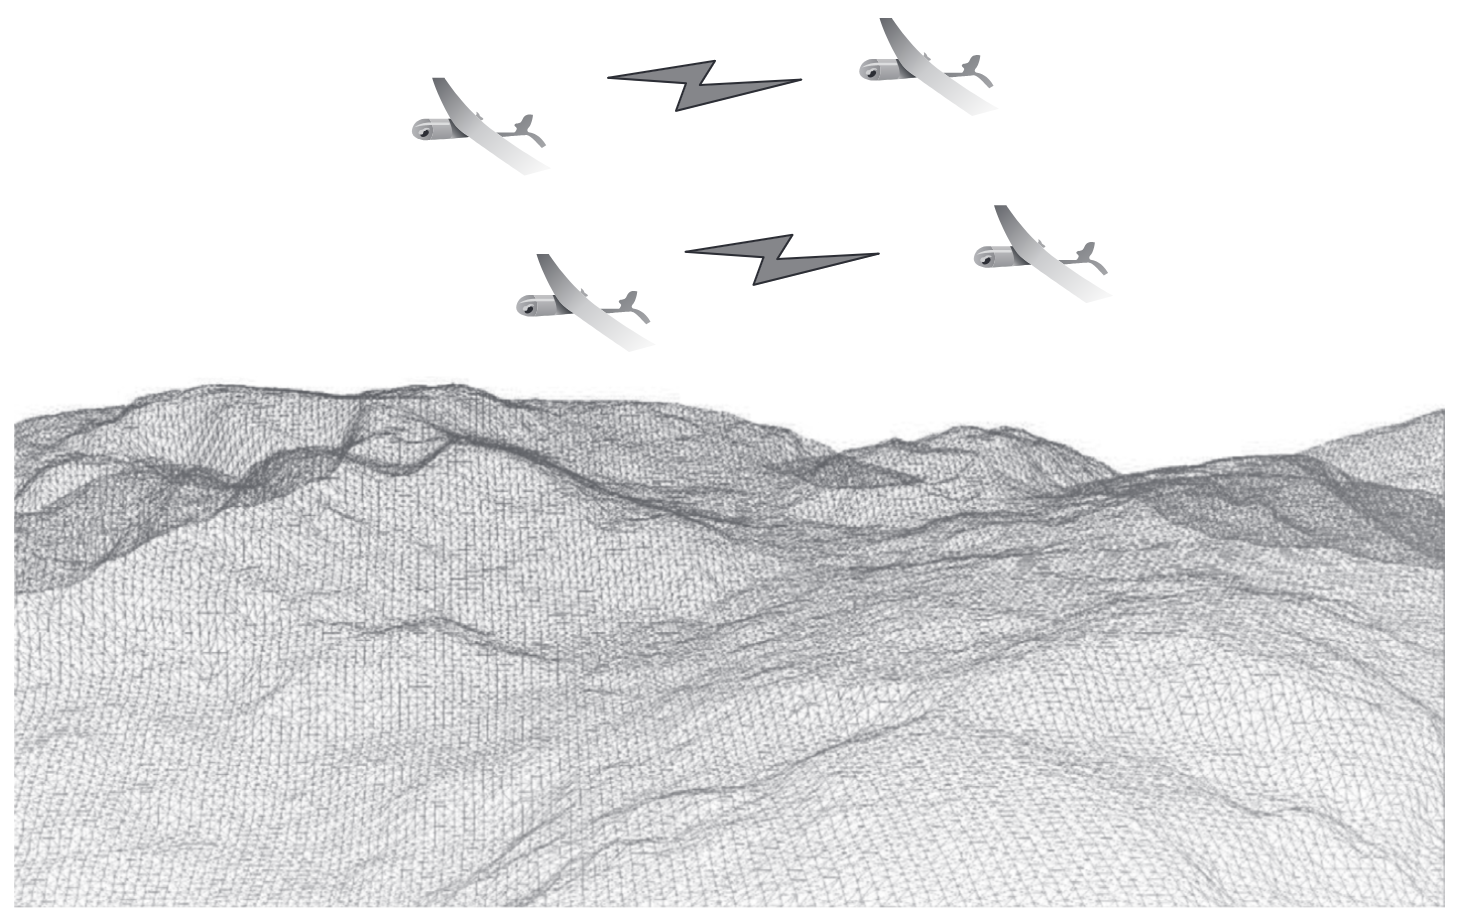
\includegraphics[width=0.75\textwidth]{figures/uav_ad_hoc_saad_textbook.png}
    \caption{Ad Hoc Configuration of \acrshort{uav} Network}
    \label{fig:uav_ad_hoc_namuduri}
\end{figure}
\acrshort{manet}s do not require the use of other network infrastructure, such as satellites or centralised servers to support the swarm of vehicles \cite{namuduri_uav_2017}, however, it's also expected that there is some assistance from terrestrial control stations as part of the network architecture \cite{namuduri_mobile_nodate}. 
Each node in the \acrshort{uav}-enabled \acrshort{manet} acts as a relay, router and terminal. 

\section{Optimisation of \texorpdfstring{\acrshort{uav}}{UAV} Communications}
%\hl{Write about what system parameters have been optimised to date in the literature, i.e., the objective and what the constraints are on that objective here}
%\\
%\hl{Compare different approaches to the problem and the key parameters that are and aren't important for different problems, e.g., energy efficiency/power consumption is a universal problem but secrecy may not be for some applications}.
%\\
%\hl{Refer to the papers saved in Zotero covering classical optimisation techniques used for systems/problems like this}
%\\
For optimal performance of an airborne network, optimisation techniques have been employed with a range of focuses for optimisation and constraints of a given system. 
The objective functions are typically mathematically derived and proven in the literature and algorithms are designed to implement them for the communications and control systems involved in airborne networks. 

Different studies focus on various aspects of airborne networks, with emphases placed on particular objectives of the system subject to a variety of relevant constraints. 
Many of these studies are presented with a joint non-convex optimisation problem that cannot be solved efficiently or easily with a standalone algorithm and thus, piecewise approaches are taken to optimise particular parameters of the system individually without violating the constraints of the overall problem. 
The main factors for optimisation that have been explored in the literature on this topic include energy efficiency \cite{zhao_energy_2023, zhang_energy-efficient_2024}, \acrshort{uav} clustering \cite{zhao_energy_2023, jeong_quantum_2025}, communication secrecy \cite{zhang_one_2025, mu_security_2021, yan_secure_2022}, platform deployment \cite{ji_joint_2023}, \acrshort{uav} trajectory \cite{zhao_energy_2023}, latency \cite{saravanan_optimizing_2024}, resource allocation\cite{ji_joint_2023} and scheduling, to name a few. 

The following subsections detail a set of focal points for optimisation and the constraints that are considered for aerial communications that have been documented to date. 
\subsection{Security \& Secrecy}
A key focus of many of these studies is the secrecy of communication and ensuring that the communications are secure between \acrshort{gu}s, \acrshort{hap}s and LAPs\cite{qin_secure_2023, zhang_one_2025, yan_secure_2022, mu_security_2021, lohan_secrecy-aware_2022}. In \cite{zhang_one_2025}, \acrshort{hap}s are deployed for communication with \acrshort{gu}s and \acrshort{uav}s are used for detection of eavesdroppers, who are referred to as "Eves" in the paper. 

\begin{figure}[ht!]
    \centering
    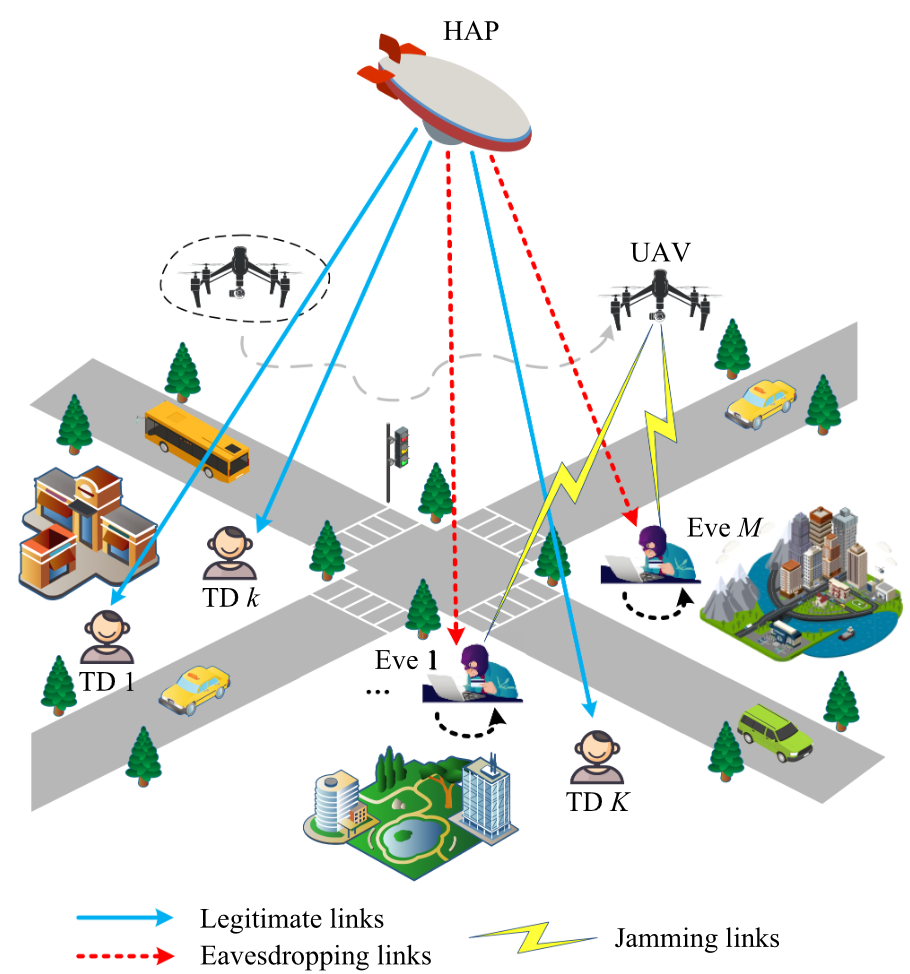
\includegraphics[width=0.7\textwidth]{figures/uav_haps_eves_diagram.png}
    \caption{Illustration of a Secure \acrshort{uav}-\acrshort{hap} Network Model}
    \label{fig:secure_uav_hap_zhang}
\end{figure}
An illustration of a secure \acrshort{uav}-\acrshort{hap} network reproduced from \cite{zhang_one_2025} is shown in Fig. \ref{fig:secure_uav_hap_zhang}, where \acrshort{uav}s are used as jammers to combat eavesdroppers and the \acrshort{hap} is used as the network provider for communication links between terrestrial \acrshort{td}s. 
The \acrshort{hap} network uses a \acrshort{uav} to interfere with the signal decoding of multiple mobile eavesdroppers. 
The \acrshort{uav}'s trajectory is dynamically adjusted and optimised based on the known locations of the eavesdroppers. 

In this study, the system's orthogonal subcarrier scheduling among \acrshort{td}s, subcarrier power allocation, \acrshort{uav} trajectory and \acrshort{hap} deployment are jointly optimised to maximise the minimum average secrecy rate (\acrshort{masr}), subject to the constraints of \acrshort{uav} mobility and \acrshort{hap} power budget.
This optimisation problem is a mixed-integer, non-convex optimisation problem, however, it is solved iteratively using successive convex approximation (\acrshort{sca}) algorithm. This is achieved by alternately optimising the \acrshort{uav} trajectory, power allocation and the subcarrier scheduling until convergence. 

Another approach to ensuring secrecy of communication is detailed in \cite{qin_secure_2023}, where the secrecy considerations are modelled as constraints in the system rather than objectives and the task computation latency, task scheduling and transmit power of legitimate users (\acrshort{lu}s) are jointly optimised for secure mobile edge computing (\acrshort{mec}). The system model is shown in Fig. \ref{fig:qin_uav_hap_mec_system_model}, which has been reproduced from \cite{qin_secure_2023}.

\begin{figure}[ht!]
    \centering
    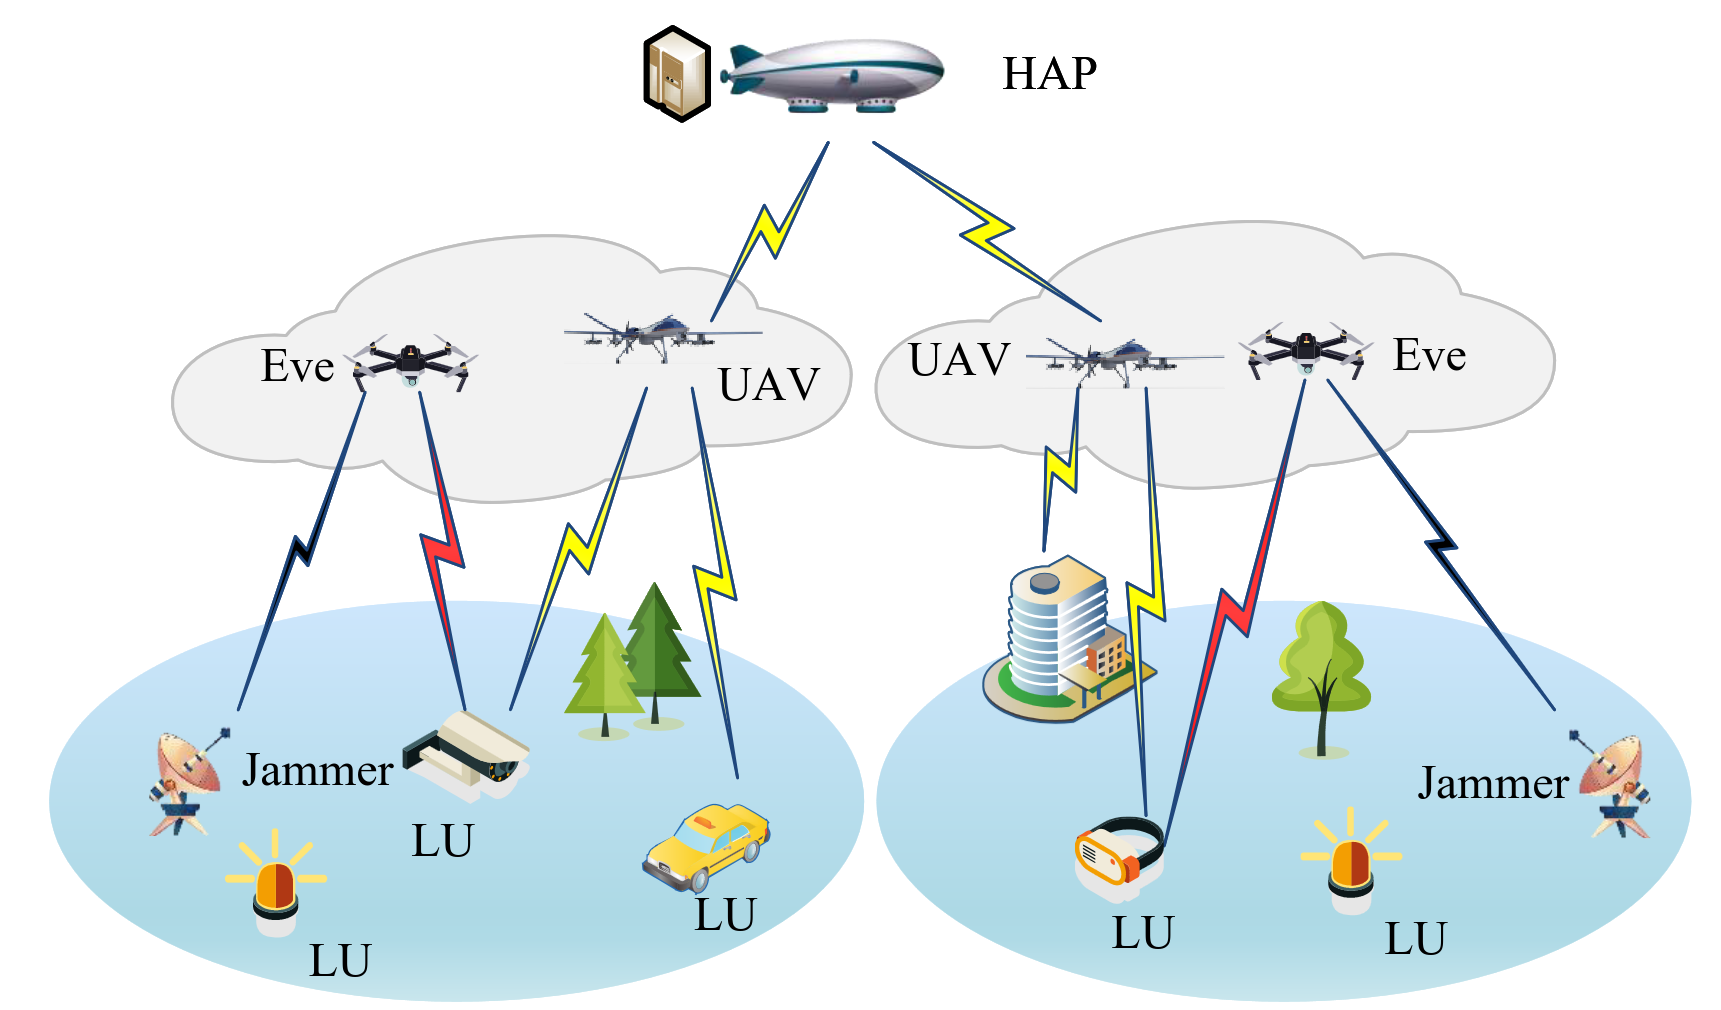
\includegraphics[width=0.75\textwidth]{figures/uav_hap_secrecy_qin.png}
    \caption{\acrshort{uav}-\acrshort{hap}-Enabled System Model for Secure \acrshort{mec}}
    \label{fig:qin_uav_hap_mec_system_model}
\end{figure}

An iterative approach is also taken for this proposed form of optimisation as in the case of \cite{zhang_one_2025}, in which the joint non-convex optimisation problem is solved by individually optimising the various parameters such that the minimum secure offloading sum rate is maximised. 
\acrshort{noma} is utilised for spectral efficiency over \acrshort{ofdm} as it allows multiple users to transmit data over the same resource block, so it supports a greater level of spectral efficiency \cite{qin_secure_2023}. 

\subsection{Energy Efficiency}
Certain studies \cite{silvirianti_energy-efficient_2022, silvirianti_layerwise_2024, zhao_energy_2023, zhang_energy-efficient_2024} focus on maximising the energy efficiency of \acrshort{uav}s in airborne networks. The importance of optimising the energy efficiency of the airborne platforms can be viewed as a universal one for the optimisation of any given \acrshort{uav} mission for networking due to the limited power capacity of LAPs, in particular that typically cannot generate any power while they're operational. 

In \cite{zhao_energy_2023}, the trajectory of \acrshort{uav}s in the network is optimised jointly with the resource allocation for the \acrshort{uav}s to maximise the energy efficiency. 
A dynamic, self-adaptive clustering algorithm based on affinity propagation and a proximal policy optimisation (\acrshort{ppo}) based deep reinforcement learning (\acrshort{drl}) algorithm are used to optimise the \acrshort{uav} clustering, trajectory planning and transmit power level of the sensing devices for providing device-to-\acrshort{uav} communication. 
In this study, \acrshort{hap}s are used as aerial \acrshort{bs}s, whereas the \acrshort{uav}s are used for the device links and communication with the \acrshort{hap}s that are providing the networking coverage. 
The simulation of the algorithm uses a scenario involving network that consists of a single \acrshort{uav} and \acrshort{hap}-\acrshort{bs} using the clustering and resource allocation algorithms to maximise the energy efficiency. 

The approach taken in \cite{zhang_energy-efficient_2024} involves the optimisation of the energy efficiency using the transmission power, \acrshort{uav} altitude and time allocation of \acrshort{hap}s and \acrshort{uav}s in the network. The architecture considered is a two-hop \acrshort{hap}-\acrshort{uav}-assisted wireless network that is serving a set of \acrshort{gu}s. 

The energy efficiency is maximised such that it does not violate the constraints of \acrshort{uav} altitude, \acrshort{uav} and \acrshort{hap} transmit power and the total operation time. 

Three algorithms are utilised to meet this objective, algorithm 1 handles the global optimal \acrshort{uav} and \acrshort{hap} transmit power, algorithm 2 handles the optimal transmit power allocation for the \acrshort{uav}s and \acrshort{hap}s alternately and algorithm 3 directly handles the energy efficiency using the optimal transmit power and allocation for the \acrshort{uav}s and \acrshort{hap}s, thus algorithm's 3 complexity and efficacy is dependent on the performance and adoption of algorithms 1 and 2 \cite{zhang_energy-efficient_2024}.

\subsection{Resource Allocation}
The allocation of resources within the network is a focus for optimisation in airborne networks. In \cite{ji_joint_2023}, a joint resource allocation problem is formulated and divided into constituent subproblems. The iterative algorithm proposed in \cite{ji_joint_2023} is sub-optimal, however, it can solve the resource allocation and \acrshort{hap} deployment optimisation problems efficiently and separately.

The resource allocation algorithm is based on the Gale-Shapely algorithm to produce a convergent solution to the two-sided matching game of the \acrshort{hap} deployment and resource allocation algorithms. 
Both algorithms are combined into a single algorithm that alternates between solving each of these problems iteratively, thus reducing it from a joint optimisation problem to two smaller subproblems for the algorithm to solve more efficiently. 

\section{Quantum Computing Techniques}
In recent years, quantum computers have been developed in an attempt to compute problems that cannot be solved as effectively, or at all, using classical computers. Different approaches to create qubits that leverage different technologies such as ion trap qubits \cite{Bruzewicz_2019}, superconducting qubits \cite{Krantz_2019}, semiconductor qubits \cite{chatterjee_semiconductor_2021} and photonic qubits \cite{Kok_2007}. 

Hybrid classical-quantum computer implementations have also been explored as feasible solutions to solving optimisation problems where some of the computation can be offloaded to one or the other means of computation depending on which method is more suitable to a portion of any given problem. 

Quantum computing can be utilised to solve complex optimisation problems. 

The two leading quantum computing paradigms are gate-based quantum computing and \acrfull{aqc} \cite{yarkoni_quantum_2022}. Gate-based quantum computing involves the application of a sequence of unitary quantum gates to a set of qubits. The states of the qubits collapse into a $\ket{0}$ or $\ket{1}$ state upon measurement. 

\acrshort{aqc} involves the preparation of a multi-qubit state as the ground state of a Hamiltonian operator. This Hamiltonian then has an adiabatic time evolution applied to it, which changes the Hamiltonian such that its ground state encodes the solution of the optimisation problem \cite{yarkoni_quantum_2022}. 
\subsection{Quantum Annealing}
Quantum annealing is a heuristic optimisation algorithm that can be used to solve combinatorial optimisation problems \cite{yarkoni_quantum_2022}.
With the use of quantum annealing, an optimisation problem can be converted into \acrlong{qubo} (\acrshort{qubo}) or Ising models \cite{jeong_quantum_2025}.
The expression for the \acrshort{qubo} problem is shown in \ref{eq:qubo}.
\begin{equation} \label{eq:qubo}
        Obj(x, Q) = x^T \cdot Q \cdot x
\end{equation}
Where $x$ is the vector of $N$ binary variables and $Q$ is the symmetric matrix defining interaction terms between the variables, which is an upper diagonal matrix  \cite{jeong_quantum_2025, yarkoni_quantum_2022}. 
In the case of the \acrshort{qubo} in \cite{jeong_quantum_2025}, the goal is to minimise $x$ in the objective function, so the \acrshort{qubo} is expressed as shown in \ref{eq:min_qubo}.
\begin{equation} \label{eq:min_qubo}
    \underset{x}{\min}\ H_{\acrshort{qubo}}(x) = x^{T} \cdot Q \cdot x
\end{equation}
The \acrshort{qubo} model can be extended to represent the binary combinatorial optimisation problem with linear and quadratic terms and, in this case, an $N \times N$ binary vector in 2 dimensions is considered. This model can be expressed as \ref{eq:lin_quad_qubo}. 
\begin{equation} \label{eq:lin_quad_qubo}
    H_{\acrshort{qubo}}(x) = \sum_{i=1}^{N} Q_{ii}x_{i} + \sum_{i=1}^{N}\sum_{j=1}^{N} Q_{ij} x_{i} x_{j}
\end{equation} 
In \cite{jeong_quantum_2025}, two quantum annealing-based algorithms are used for the optimisation of \acrshort{uav} clustering and for sub-channel assignment and power allocation. This algorithm is described pictorially in Fig. \ref{fig:quantum_annealing_uav_jeong}, which has been reproduced from \cite{jeong_quantum_2025}. 

\begin{figure}[ht]
    \centering
    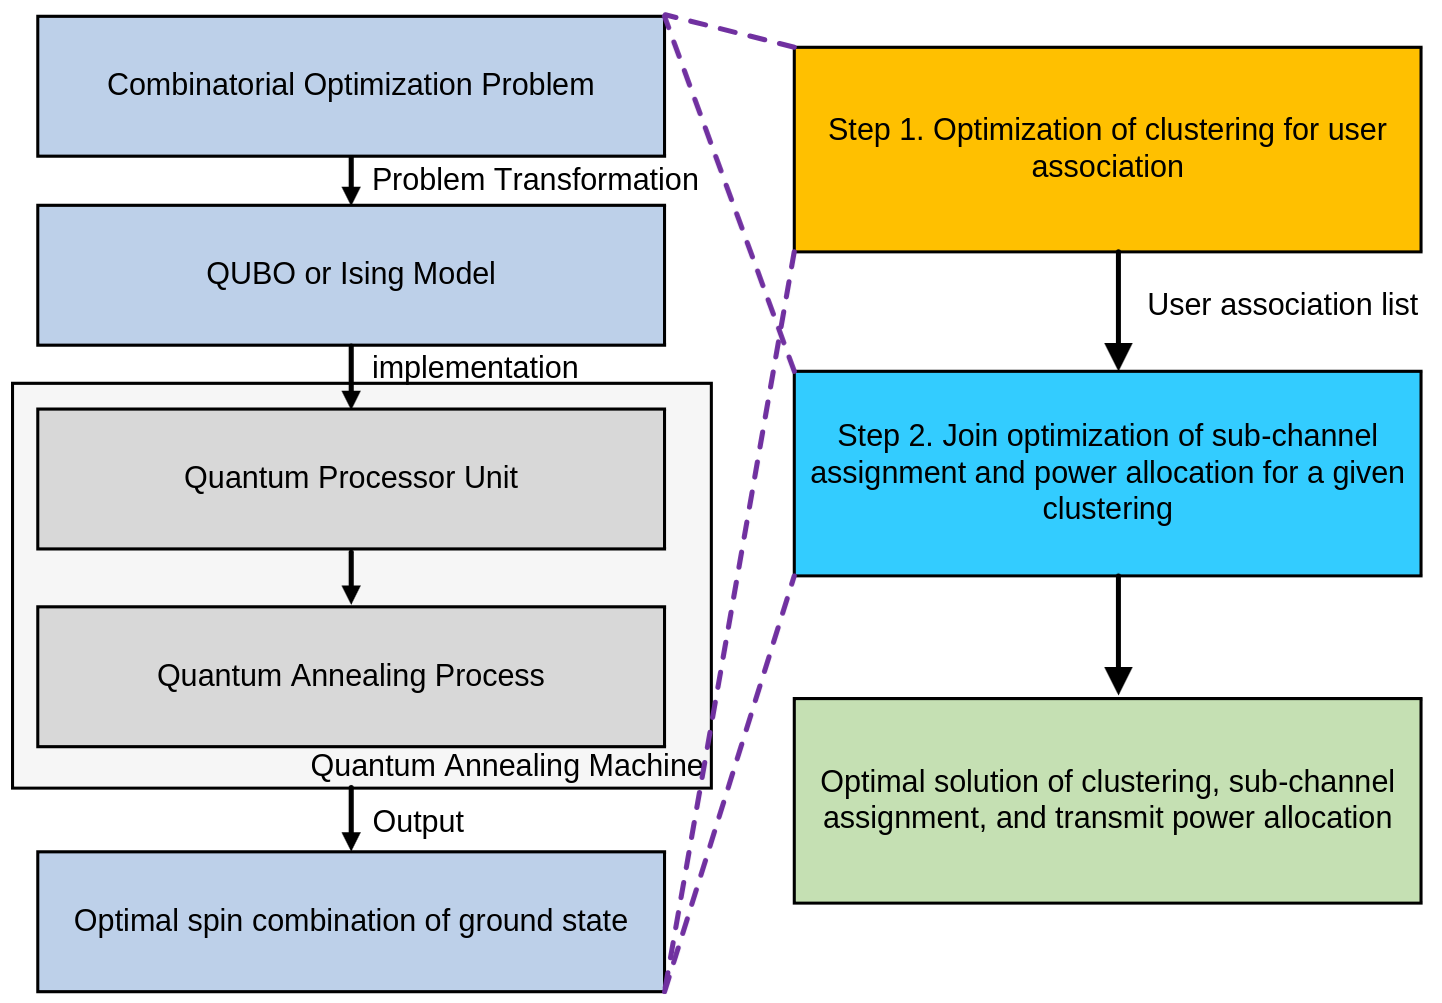
\includegraphics[width=1\textwidth]{figures/quantum_annealing_uav_algorithm.png}
    \caption{Quantum Annealing Based Algorithms for Optimisation of Clustering, Sub-Channel Assignment and Power Allocation}
    \label{fig:quantum_annealing_uav_jeong}
\end{figure}
In \cite{jeong_quantum_2025}, a quantum annealing-based clustering algorithm with a constrained quadratic model (\acrshort{cqm}) is used to optimise a binary variable that indicates if a \acrshort{uav} is associated with a \acrshort{gu} or not. 
The algorithm takes the locations of the \acrshort{gu}s and \acrshort{uav}s and builds the \acrshort{cqm} object. It then maps the cost function for optimising the \acrshort{uav} and \acrshort{gu} clustering to a \acrshort{qubo} Hamiltonian that is energy-based for use with D-Wave's quantum annealing machine, runs the \acrshort{cqm} sampler and then returns the optimal spin combination for the association of \acrshort{gu}s with \acrshort{uav}s for clustering. 
This algorithms provides the clustering configuration for the \acrshort{uav}s for the set of \acrshort{gu}s. 
The next algorithm handles the joint optimisation of the power allocation and sub-channel assignment for this clustering configuration that has been determined. 

The proposed quantum annealing based algorithm using a D-Wave hybrid \acrshort{qubo} solver outperformed classical K-means, simulated annealing \cite{kirkpatrick_optimization_nodate} and steepest descent \cite{battiti_first-_1992} algorithms in terms of maximisation of the sum rate, measured in Mbps. 
This increase in the quantum annealing based algorithms' performance also scaled better than the pre-existing algorithms with increases in the number of \acrshort{gu}s. 
The simulation time was also faster and remained low for increasing numbers of \acrshort{uav}s where the simulation time of the other algorithms began to increase for increasing numbers of \acrshort{uav}s with the proposed scenarios presented in the paper.

The optimisation algorithms that were compared against the proposed algorithm were not specially designed for \acrshort{uav} clustering or airborne communications and were published in the 1980s and 1990s. 
While this does not infringe on the validity of these methodologies, comparisons against newer algorithms that have been specifically designed for this problem could reflect its efficacy more accurately. 

\subsection{Quantum Embedding \& \texorpdfstring{\acrshort{drl}}{DRL}}
Quantum embedding is a process in which classical data can be stored and encoded into quantum states by passing a vector of data through a quantum circuit and storing the data upon measurement once this state has undergone time evolution through the circuit. 
The encoding operation acting on an input vector of classical data $x$ with $N$ elements can be mapped to a quantum state such that the input data is mapped to a quantum state as shown in \ref{eq:encoding_op}.
\begin{equation} \label{eq:encoding_op}
    S_x : \begin{Bmatrix}
        x_n
    \end{Bmatrix}_{n=1}^{N} \xrightarrow[]{} \begin{Bmatrix}
        \ket{\psi}
    \end{Bmatrix}_{n=1}^{N}
\end{equation}
Where $\ket{\psi}$ denotes the $n^{th}$ quantum state \cite{silvirianti_layerwise_2024}. 
Different encoding techniques can be used for quantum embedding \cite{munikote_comparing_2024, rath_quantum_2023}.
Basis encoding directly maps classical bits to qubits as shown in \ref{eq:basis_encoding}. 
\begin{equation} \label{eq:basis_encoding}
    \ket{x} = \ket{b_1} \otimes \ket{b_2} \dots \ket{b_n}
\end{equation}
Where $\ket{b_i}$ are the binary digits of $\textbf{x}$. 
Basis encoding requires many qubits to encode data as a result of it being a one-to-one mapping scheme, thus, it scales poorly for increasing dataset sizes. 

Superposition encoding is a technique that involves encoding classical data as a superposition of multiple states at once and it represents a quantum state as a linear combination of basis states, illustrated by the example shown by \ref{eq:eg_superposition_encoding}. 
\begin{equation} \label{eq:eg_superposition_encoding}
    \ket{101} \xrightarrow{} \alpha\ket{000} + \beta\ket{010} + \gamma\ket{001}
\end{equation}
Angle encoding encodes classical data in the relative phase between different basis states with the use of phase rotation gates, i.e., $R_{X}(\theta)$, $R_{Y}(\theta)$ and $R_{Z}(\theta)$. 
This encoding scheme requires $n$ qubits for $n$ data points being encoded into those qubits, which can lead to deep quantum circuits for large values of $n$.

Amplitude encoding involves encoding classical information into the amplitudes of a quantum state and it can be expressed mathematically as shown in \ref{eq:amplitude_encoding_equation}. 
\begin{equation} \label{eq:amplitude_encoding_equation}
    \ket{x} = \frac{x_1}{\sqrt{\sum_{i=1}^{n}}x_i^2}\ket{0} + \frac{x_2}{\sqrt{\sum_{i=1}^{n}}x_i^2}\ket{1} + \dots + \frac{x_n}{\sqrt{\sum_{i=1}^{n}}x_i^2}\ket{n-1}
\end{equation}
Amplitude encoding requires a smaller number of qubits compared to the other major encoding schemes, however, it also requires a novel preparation protocol and the use of quantum tomography to determine what the probability amplitudes are as a result of the encoding process \cite{munikote_comparing_2024, rath_quantum_2023}.

Generally, several layers of quantum encoding are required for the quantum embedding process. 
Different approaches can be taken to obtain the classical values after the embedding process in which all of the data is obtained once all of the quantum embedding layers have encoded all of the classical information into quantum states, however, in \cite{silvirianti_layerwise_2024}, measurements are taken after each layer to employ local loss training. 

\acrshort{drl} is a branch of machine learning that combines the concepts of deep learning and reinforcement learning and this integration enables the agents interacting with the environment in \acrshort{drl} algorithms to be able to handle high-dimensional input spaces, such as the environmental, secrecy and energy considerations of a network of \acrshort{uav}s. 

Generally, \acrshort{drl} algorithms work by using a learning agent to interact with a training environment by taking an action based on the observation of the current state. 
It then moves onto the next state. 
The optimal action is taken at discrete intervals under a particular policy to ensure the maximum reward for the network is attained and higher rewards are obtained over time. 
An episode refers to the single-chain agent interaction and the interaction experience from each episode is stored in a memory experience replay, which is used to update the policy until it converges into the optimal policy \cite{silvirianti_layerwise_2024}. 

The memory experience replay (\acrshort{mer}), shown in the \acrshort{lqdrl} framework pictured in Fig. \ref{fig:lqdrl_framework_silvirianti} stores the following parameters: action $a$ taken by agent, observed state $s$ of the system at time $t$, the reward $r$ for the action taken and $s'$ refers to the next state at time $t+1$.

The layerwise quantum deep reinforcement learning (\acrshort{lqdrl}) framework refers to the integration of the layerwise quantum embedding with local loss training with the \acrshort{drl}-based actor-critic network. 

The proposed framework used in \cite{silvirianti_layerwise_2024} for the \acrshort{lqdrl} methodology is displayed in Fig. \ref{fig:lqdrl_framework_silvirianti}.

\begin{figure}[ht]
    \centering
    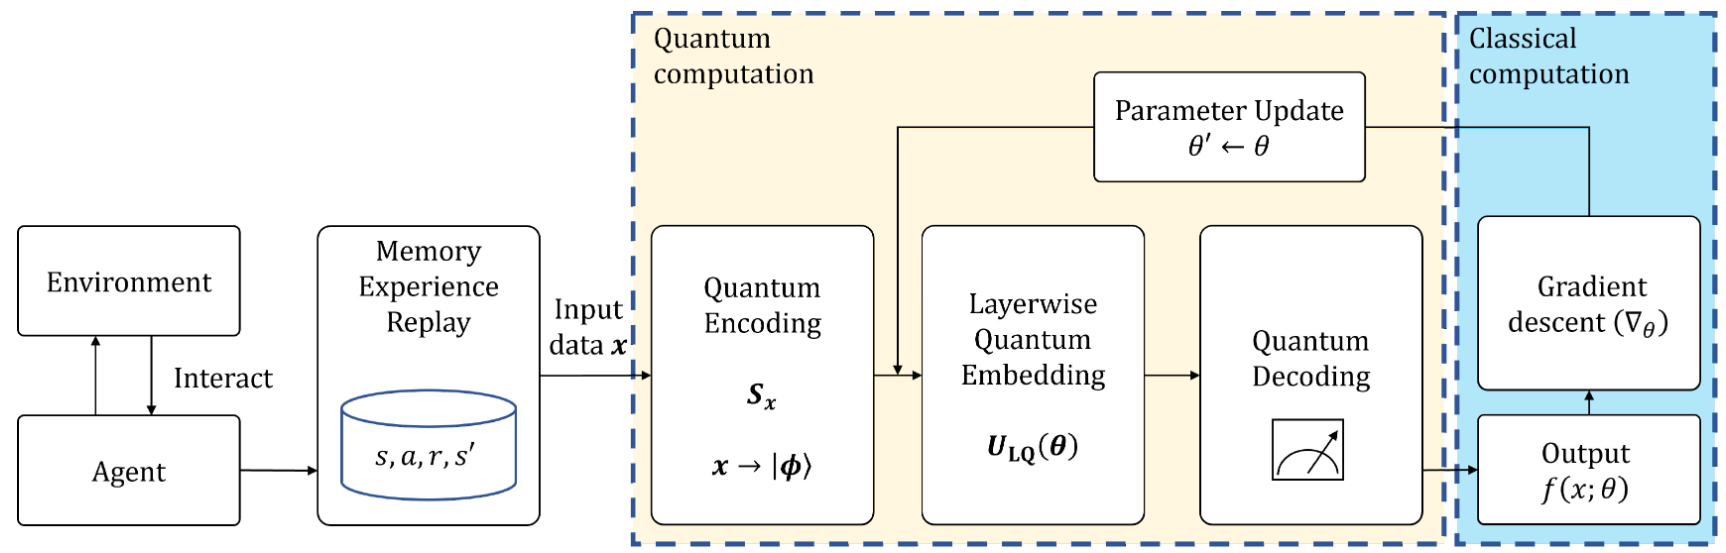
\includegraphics[width=1\textwidth]{figures/lq_drl_framework_silviratani_et_al.png}
    \caption{\acrshort{lqdrl} Framework Proposed by Silvirianti et. al (2025)}
    \label{fig:lqdrl_framework_silvirianti}
\end{figure}
It can be seen in Fig. \ref{fig:lqdrl_framework_silvirianti} that a hybrid approach is taken for computing the optimal parameters for the \acrshort{drl} algorithm, i.e., part of the computation is performed using quantum gates and the other part is performed using classical computing methods, however, both portions of the overall system rely on one another to perform \acrshort{drl}. 

The study involved the use of a \acrshort{drl} that employs a deep neural network to enable the agent to learn in a high-dimensional, continuous space and not a discrete one, which is typical for \acrshort{drl} algorithms. 

The optimal action policy is selected by the actor network and the critic network evaluates the quality of this selected policy by referring to the maximum Q-values at that given layer. The Q-values represent a value given a particular action and state at a given time.
As they are directly related to the rewards given for particular actions, they must be updated over time as opposed to being kept the same from iteration to iteration \cite{skolik_quantum_2022}. 

The use of quantum embedding and measurement for each layer was performed for encoding all of the data into quantum states with the use of an ansatz for quantum embedding, i.e. a quantum circuit. 
There is a decoding operator that acts on the quantum state for measurement to collapse the quantum information into classical information, which then provides an input for a gradient descent optimisation algorithm that updates parameters for the next layer to be embedded and subsequently decoded. 
The decoding operation is then used to calculate the value of the local loss for each iteration of this process and each measurement operation is performed $K_{shot}$ times. The local loss is a measure of the difference between the decoded output and the desired output averaged over $N_{data}$ times, where $N_{data}$ is the size of the encoded data. 

The proposed ansatz for the layerwise quantum embedding in this study is shown in Fig. \ref{fig:lqdrl_ansatz_silvirianti}, which has been reproduced from \cite{silvirianti_layerwise_2024}. 

\begin{figure}[ht]
    \centering
    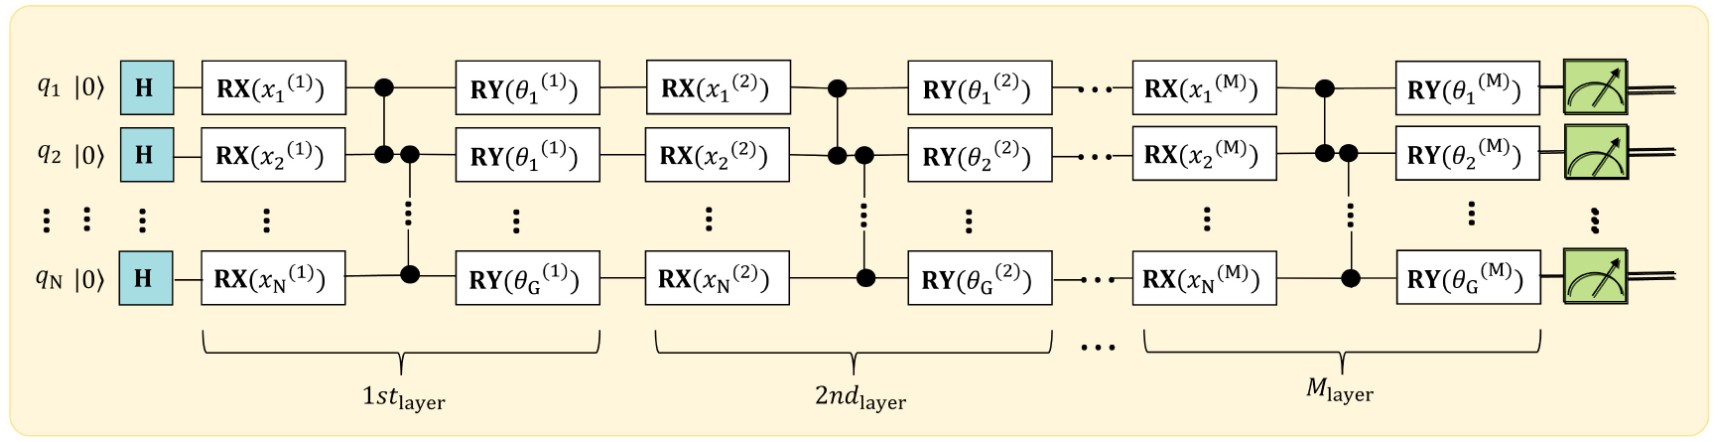
\includegraphics[width=1\textwidth]{figures/lq_drl_ansatz.png}
    \caption{Ansatz Used for Layerwise Quantum Embedding Proposed by Silvirianti et. al (2025)}
    \label{fig:lqdrl_ansatz_silvirianti}
\end{figure}
The layerwise quantum embedding process is performed for the actor and critic networks. 

The employed \acrshort{lqdrl} scheme was used to jointly optimise the \acrshort{uav} trajectory planning, transmit power allocation and \acrshort{noma} user grouping. 

The scenario considered for evaluating the performance of the algorithm involved a single \acrshort{uav} in three-dimensional space, with full power $E_{max}$, acting as an aerial \acrshort{bs} to provide downlink coverage serving $K$ \acrshort{gu}s that were distributed randomly over the horizontal plane, i.e. in two dimensions and moving at constant speeds.  
The authors formulated energy consumption models, \acrshort{noma} channel grouping, transmission power models, a noise and interference model and subsequently formulated an objective function that aimed to maximise the energy efficiency of the \acrshort{uav} network subject to the following constraints:
\begin{itemize}
    \item The total maximum transmit power of the \acrshort{uav} must not be exceeded by the total allocated power for the \acrshort{gu}s in a \acrshort{noma} group.
    \item The range of the allocated power coefficient for each user must not be exceeded and must fall between 0 and 1 .
    \item Higher transmission power must be allocated to \acrshort{gu}s with a lower channel gain.
    \item The minimum threshold data rate must be exceeded by the achievable data rate of any \acrshort{gu} within a given group at a particular time
    \item The \acrshort{uav} must remain within its maximum allowed co-ordinates in Cartesian co-ordinates.
\end{itemize}
The authors formulated a state space for the \acrshort{uav} in which the location, remaining energy to consume and the states of the \acrshort{gu}s are considered with $(2K + 4)$ state space dimensions, where $K$ denotes the number of \acrshort{gu}s. 

An action space was also formulated based on the objective problem of jointly optimising the \acrshort{uav} trajectory, \acrshort{noma} user grouping and power allocation. 
Action $a$ considered the following actions:
\begin{itemize}
    \item \textbf{\acrshort{uav} Trajectory} controlled by the velocity of the \acrshort{uav} and related to it's maneuvre.
    \item \textbf{\acrshort{noma} User Grouping} to address every possible GU clustering outcome and its objective is reward maximisation. 
    \item \textbf{Dynamic Power Allocation} which orders the transmit power allocations based on the highest to lowest channel gains for all of the \acrshort{gu}s.
\end{itemize}

The action space has 5 dimensions in total.

The reward $r$ is determined based on the energy efficiency $\eta(t)$ of a given episode and this is the value that's assigned as a reward if the energy efficiency optimisation is met, otherwise a value of $0$ is assigned for reward $r$. 

The \acrshort{lqdrl} algorithm used in \cite{silvirianti_layerwise_2024} demonstrated that the \acrshort{lqdrl} algorithm had higher effective dimensionality compared to a classical \acrshort{drl} approach. 
The layer loss was also shown to decrease in magnitude for each layer. 
The energy efficiency, critic and actor loss also decreased substantially, with improvements being demonstrated to occur for each layer. 